\chapter{Basic Algorithms (Quantum Primitives)}\label{ch:sec02}

This chapter introduces four fundamental quantum primitives: Deutsch's
algorithm, Grover's algorithm, the quantum Fourier transform (QFT), and quantum
phase estimation (QPE).

\section{Deutsch's algorithm}\label{sec:sec02-deutsch}

Consider two boxes, each containing either an apple or an orange
(\cref{fig:sec02-boxes}). We wish to decide whether the two boxes contain the
same type of fruit, without needing to tell \emph{which} type. It is impossible
to answer whether the fruit types are the same without knowing the types.

\begin{figure}[ht]
  \centering
  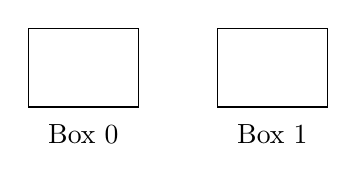
\begin{tikzpicture}
    \draw (0,0) rectangle (1.4,1); \node at (0.7,-0.35) {Box $0$};
    \draw (2.4,0) rectangle (3.8,1); \node at (3.1,-0.35) {Box $1$};
  \end{tikzpicture}
  \caption{Two boxes, each containing an apple or an orange.}
  \label{fig:sec02-boxes}
\end{figure}

Abstractly, consider a Boolean function $f : \{0,1\} \to \{0,1\}$, and ask
whether $f(0) = f(1)$ or $f(0) \neq f(1)$.

\paragraph{Quantum oracle.}
A quantum fruit-checker assumes access to $f$ via the quantum oracle
\begin{equation}
  U_f\ket{x, y} = \ket{x,\, y \oplus f(x)}, \qquad x, y \in \{0,1\}.
\end{equation}
A classical fruit-checker can only query $U_f$ in the computational basis, as
$U_f\ket{0,0} = \ket{0, f(0)}$ and $U_f\ket{1,0} = \ket{1, f(1)}$; after two
queries it measures the qubit to obtain the deterministic outcomes $f(0)$ and
$f(1)$, then answers whether $f(0) = f(1)$. A quantum fruit-checker can instead
apply $U_f$ to a linear combination of computational-basis states. One checks
that $U_f$ is unitary: for $x', x, y', y \in \{0,1\}$,
\begin{equation}
  \bra{x', y'} U_f\dg U_f \ket{x, y}
  = \braket{x', y' \oplus f(x') \,|\, x, y \oplus f(x)}
  = \delta_{x x'}\delta_{y y'},
\end{equation}
so $U_f\dg U_f = I$.

\paragraph{Phase kickback.}
With query access to a Boolean function $f : \{0,1\}^n \to \{0,1\}$, the oracle
can be turned into a phase, $U_f\ket{x} = (-1)^{f(x)}\ket{x}$. Take
$\ket{y} = \ket{-} = \tfrac{1}{\sqrt{2}}(\ket{0} - \ket{1})$; then
\begin{equation}
  U_f\ket{x, -} = \tfrac{1}{\sqrt{2}}\bigl(\ket{x, f(x)} - \ket{x, 1 \oplus f(x)}\bigr)
  = (-1)^{f(x)}\ket{x, -}.
  \label{eq:sec02-kickback}
\end{equation}
Since $\ket{-} = HX\ket{0}$, \eqref{eq:sec02-kickback} can be interpreted as
$(I \otimes XH)\, U_f\, (I \otimes HX)\ket{x, 0} = (-1)^{f(x)}\ket{x, 0}$, where
qubit $1$ does not change. Thus, for qubit $0$, there is an effective unitary
$\widehat{U}_f\ket{x} = (-1)^{f(x)}\ket{x}$ (neglecting qubit $1$).

The quantum circuit for Deutsch's algorithm is shown in
\cref{fig:sec02-deutsch}. Equivalently,
\begin{align}
  \ket{0,1} &\xrightarrow{H \otimes H} \ket{+, -}
    = \tfrac{1}{\sqrt{2}}(\ket{0} + \ket{1}) \otimes \ket{-} \\
  &\xrightarrow{U_f} \tfrac{1}{\sqrt{2}}\bigl((-1)^{f(0)}\ket{0} + (-1)^{f(1)}\ket{1}\bigr) \otimes \ket{-} \\
  &\xrightarrow{H \otimes I} \tfrac{1}{2}\bigl((-1)^{f(0)} + (-1)^{f(1)}\bigr)\ket{0, -}
    + \tfrac{1}{2}\bigl((-1)^{f(0)} - (-1)^{f(1)}\bigr)\ket{1, -}.
\end{align}
Measuring qubit $0$: if $f(0) = f(1)$ the final state is $\pm\ket{0, -}$, giving
outcome $0$ deterministically; if $f(0) \neq f(1)$ it is $\pm\ket{1, -}$, giving
outcome $1$ deterministically. Hence a single query to $U_f$ suffices to
determine whether $f(0) = f(1)$.

\begin{figure}[ht]
  \centering
  \begin{quantikz}
    \lstick{$\ket{0}$} & \gate{H} & \gate[2]{U_f} & \gate{H} & \meter{} \\
    \lstick{$\ket{1}$} & \gate{H} &               & \qw      & \qw
  \end{quantikz}
  \caption{Quantum circuit for Deutsch's algorithm. Note that the single-qubit
    measurement distinguishes it from a classical checker.}
  \label{fig:sec02-deutsch}
\end{figure}

\paragraph{Deutsch--Jozsa.}
The Deutsch--Jozsa algorithm is the $n$-qubit version of Deutsch's algorithm.
Given $N = 2^n$ boxes, each with an orange or an apple, and promised that either
(i) all boxes contain the same type of fruit, or (ii) exactly half the boxes
contain apples and the other half oranges, the algorithm decides which case
holds with gate complexity $\bigo(n)$.

\paragraph{Qiskit implementation.}
\Cref{fig:sec02-qiskit-circ} shows the constant and balanced circuits and the
Deutsch circuit for the balanced case; \cref{fig:sec02-qiskit-bars} shows the
measured output probabilities on a simulator and on an IBMQ device.

\begin{figure}[ht]
  \centering
  \begin{quantikz}
    \lstick{$q_0$} & \qw      & \\
    \lstick{$q_1$} & \gate{X} &
  \end{quantikz}
  \quad\raisebox{-3ex}{\small constant}\qquad
  \begin{quantikz}
    \lstick{$q_0$} & \ctrl{1} & \\
    \lstick{$q_1$} & \targ{}  &
  \end{quantikz}
  \quad\raisebox{-3ex}{\small balanced}\qquad
  \begin{quantikz}
    \lstick{$q_0$} & \gate{H} & \ctrl{1} & \gate{H} & \meter{} \\
    \lstick{$q_1$} & \gate{X} & \targ{}  & \qw      & \qw
  \end{quantikz}
  \caption{Qiskit circuits: constant and balanced oracles, and Deutsch's
    algorithm for the balanced circuit.}
  \label{fig:sec02-qiskit-circ}
\end{figure}

\begin{figure}[ht]
  \centering
  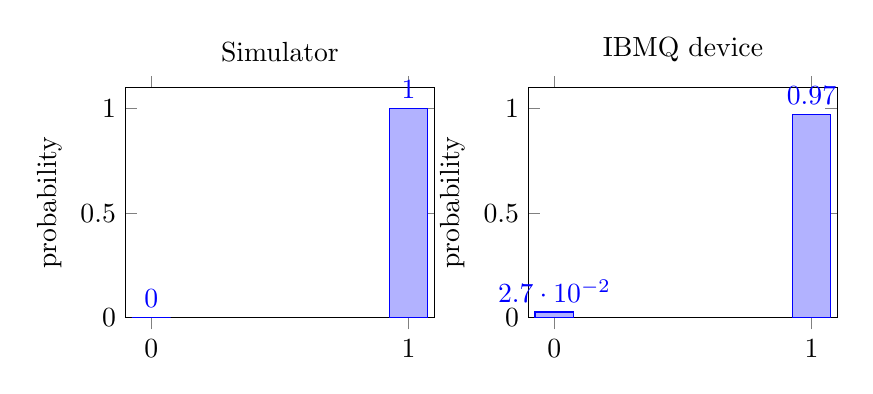
\begin{tikzpicture}
    \begin{axis}[
      name=sim, width=5.5cm, height=4.5cm, ybar, ymin=0, ymax=1.1,
      symbolic x coords={0,1}, xtick=data, ylabel={probability},
      title={Simulator}, nodes near coords, bar width=14pt]
      \addplot coordinates {(0,0) (1,1.0)};
    \end{axis}
    \begin{axis}[
      at={(sim.east)}, anchor=west, xshift=1.2cm,
      width=5.5cm, height=4.5cm, ybar, ymin=0, ymax=1.1,
      symbolic x coords={0,1}, xtick=data, ylabel={probability},
      title={IBMQ device}, nodes near coords, bar width=14pt]
      \addplot coordinates {(0,0.027) (1,0.973)};
    \end{axis}
  \end{tikzpicture}
  \caption{Measured output probabilities for the balanced case: an ideal
    simulator (left) and an IBMQ device (right).}
  \label{fig:sec02-qiskit-bars}
\end{figure}

\section{Grover's algorithm and amplitude amplification}\label{sec:sec02-grover}

\paragraph{Unstructured search.}
Assume $N = 2^n$ boxes, only one of which contains an orange while each of the
others contains an apple; the goal is to find the box containing the orange.
Formally, given a Boolean function $f : \{0,1\}^n \to \{0,1\}$ and assuming there
exists a unique $x_0$ with $f(x_0) = 1$, find $x_0$. Classically, in the worst
case this needs to open $N - 1$ boxes. The quantum algorithm (Grover's
algorithm) relies on an oracle
\begin{equation}
  U_f\ket{x, y} = \ket{x,\, y \oplus f(x)}, \qquad x \in \{0,1\}^n,\ y \in \{0,1\},
\end{equation}
and can find $x_0$ in $\bigo(\sqrt{N})$ queries.

We start from the initial state
$\ket{\psi_0} = \tfrac{1}{\sqrt{N}}\sum_{x \in [N]} \ket{x}$, which can be
prepared using Hadamard gates as
$\ket{\psi_0} = H^{\otimes n}\ket{0^n} = (H\ket{0})^{\otimes n}$, with
$H\ket{0} = \ket{+}$. We would like to amplify the desired amplitude for
$\ket{x_0}$ from $\tfrac{1}{\sqrt{N}}$ to $\sqrt{p} = \Omega(1)$; this requires
$\bigo(\sqrt{N})$ queries to $U_f$. We then measure the final state in the
computational basis to obtain some output $\ket{x}$, and check whether $x = x_0$
by applying another query, $U_f\ket{x, 0} = \ket{x, f(x)}$.

\paragraph{Reflection operators.}
The first step is to turn $U_f$ into a phase kickback: taking $\ket{y} = \ket{-}$,
for any $x \in \{0,1\}^n$,
\begin{equation}
  U_f\ket{x, -} = (-1)^{f(x)}\ket{x, -}.
\end{equation}
Any quantum state $\ket{\psi}$ can be decomposed as
$\ket{\psi} = \alpha\ket{x_0} + \beta\ket{\psi^\perp}$, where
$\ket{\psi^\perp}$ is the component orthogonal to $\ket{x_0}$, i.e.
$\braket{\psi^\perp | x_0} = 0$. Then
\begin{equation}
  U_f\ket{\psi} \otimes \ket{-} = \bigl(-\alpha\ket{x_0} + \beta\ket{\psi^\perp}\bigr) \otimes \ket{-}.
\end{equation}
Discarding the $\ket{-}$, which is unchanged, we obtain an $n$-qubit unitary
$R_{x_0}$ with
\begin{equation}
  R_{x_0}\bigl(\alpha\ket{x_0} + \beta\ket{\psi^\perp}\bigr) = -\alpha\ket{x_0} + \beta\ket{\psi^\perp}.
\end{equation}
Therefore $R_{x_0}$ is a reflection operator across the hyperplane orthogonal to
$\ket{x_0}$, i.e.\ the Householder reflector
\begin{equation}
  R_{x_0} = I - 2\ket{x_0}\bra{x_0}.
\end{equation}
Write $\ket{\psi_0} = \sin\tfrac{\theta}{2}\ket{x_0} + \cos\tfrac{\theta}{2}\ket{\psi_0^\perp}$
with $\theta = 2\arcsin\tfrac{1}{\sqrt{N}} \approx \tfrac{2}{\sqrt{N}}$, where
$\ket{\psi_0^\perp} = \tfrac{1}{\sqrt{N-1}}\sum_{x \neq x_0}\ket{x}$ is a
normalized state orthogonal to $\ket{x_0}$. Note that
$R_{x_0}\ket{\psi_0} = -\sin\tfrac{\theta}{2}\ket{x_0} + \cos\tfrac{\theta}{2}\ket{\psi_0^\perp}$,
so $\operatorname{span}\{\ket{x_0}, \ket{\psi_0^\perp}\}$ is an invariant subspace
of $R_{x_0}$.

We also consider another Householder reflector with respect to $\ket{\psi_0}$;
for later convenience we add a global phase factor $-1$,
\begin{equation}
  R_{\psi_0} = -\bigl(I - 2\ket{\psi_0}\bra{\psi_0}\bigr).
\end{equation}
A direct computation shows
\begin{align}
  R_{\psi_0} R_{x_0}\ket{\psi_0}
  &= R_{\psi_0}\Bigl(\ket{\psi_0} - 2\sin\tfrac{\theta}{2}\ket{x_0}\Bigr) \notag\\
  &= \sin\tfrac{3\theta}{2}\ket{x_0} + \cos\tfrac{3\theta}{2}\ket{\psi_0^\perp}.
\end{align}
So define the \emph{Grover operator} $G = R_{\psi_0} R_{x_0}$ as the product of
two reflection operators; it amplifies the angle from $\tfrac{\theta}{2}$ to
$\tfrac{3\theta}{2}$ (\cref{fig:sec02-grover-geom}).

\begin{figure}[ht]
  \centering
  \begin{tikzpicture}[scale=1.0, >={Stealth[]}]
    \draw[->] (-0.3,0) -- (4,0) node[right] {$\ket{x_0}$};
    \draw[->] (0,-0.3) -- (0,4) node[above] {$\ket{\psi_0^\perp}$};
    \draw[->,thick] (0,0) -- (75:3.4) node[above] {$\ket{\psi_0}$};
    \draw[->,thick,green!60!black] (0,0) -- (105:3.4) node[above left] {$R_{x_0}\ket{\psi_0}$};
    \draw[->,thick,orange] (0,0) -- (45:3.4) node[right] {$R_{\psi_0} R_{x_0}\ket{\psi_0}$};
    \draw (0,1.1) arc (90:75:1.1) node[midway,above] {\scriptsize$\tfrac{\theta}{2}$};
    \draw (75:1.35) arc (75:45:1.35) node[midway,right] {\scriptsize$\theta$};
    \draw (45:1.7) arc (45:90:1.7);
    \node at (67:2.2) {\scriptsize$\tfrac{3\theta}{2}$};
  \end{tikzpicture}
  \caption{One Grover iteration rotates the state by an angle $\theta$ toward
    $\ket{x_0}$.}
  \label{fig:sec02-grover-geom}
\end{figure}

Applying the Grover operator $k$ times, we obtain
\begin{equation}
  G^k\ket{\psi_0} = \sin\!\Bigl(\tfrac{2k+1}{2}\theta\Bigr)\ket{x_0}
    + \cos\!\Bigl(\tfrac{2k+1}{2}\theta\Bigr)\ket{\psi_0^\perp}.
\end{equation}
If $\sin\!\bigl(\tfrac{2k+1}{2}\theta\bigr) \approx 1$, we need
$k \approx \tfrac{\pi}{2\theta} - \tfrac{1}{2} \approx \tfrac{\sqrt{N}}{4}\pi$.
Thus Grover's algorithm can solve the unstructured search with
$\bigo(\sqrt{N})$ queries to $U_f$.

\paragraph{Alternative derivation.}
In the orthonormal basis $B = \{\ket{x_0}, \ket{\psi_0^\perp}\}$, the matrix
representation of $R_{x_0} = I - 2\ket{x_0}\bra{x_0}$ is
$[R_{x_0}]_B = \begin{psmallmatrix} -1 & 0 \\ 0 & 1 \end{psmallmatrix}$, and the
matrix representation of $R_{\psi_0} = 2\ket{\psi_0}\bra{\psi_0} - I$ (the Grover
diffusion operator) is
\begin{equation}
  [R_{\psi_0}]_B = \begin{pmatrix} 2a^2 - 1 & 2a\sqrt{1-a^2} \\ 2a\sqrt{1-a^2} & 1 - 2a^2 \end{pmatrix}
  = \begin{pmatrix} -\cos\theta & \sin\theta \\ \sin\theta & \cos\theta \end{pmatrix},
\end{equation}
where $a = \sin\tfrac{\theta}{2} = \tfrac{1}{\sqrt{N}}$. Therefore the matrix
representation of $G = R_{\psi_0} R_{x_0}$ is
\begin{equation}
  [G]_B = \begin{pmatrix} \cos\theta & \sin\theta \\ -\sin\theta & \cos\theta \end{pmatrix},
\end{equation}
i.e.\ $G$ is a rotation matrix with respect to $\Hilb = \operatorname{span} B$.
The initial vector is
$[\ket{\psi_0}]_B = \begin{psmallmatrix} \sin\tfrac{\theta}{2} \\ \cos\tfrac{\theta}{2} \end{psmallmatrix}$,
so Grover's search can be applied via $G^k$ for $k \approx \tfrac{\pi\sqrt{N}}{4}$
times.

To implement Grover's algorithm we need an implementation of $R_{\psi_0}$; note
that
\begin{equation}
  R_{\psi_0} = H^{\otimes n}\bigl(2\ket{0^n}\bra{0^n} - I\bigr) H^{\otimes n},
\end{equation}
which can be implemented via a circuit using one ancilla qubit
(\cref{fig:sec02-rpsi}). Here the controlled-NOT gate is only active if the
system qubits are in the $\ket{0^{\otimes n}}$ state, and the signal qubit
$\ket{-}$ only changes up to a sign ($R_{\psi_0}\ket{-} = \ket{-}$,
$R_{\psi_0}\ket{-} = -\ket{-}$ with $S \perp \ket{-}$), so it can be reused for
both $R_{\psi_0}$ and $R_{x_0}$.

\begin{figure}[ht]
  \centering
  \begin{quantikz}
    \lstick{$\ket{0}$} & \gate{H} & \gate{X} & \gate{Z} & \gate{X} & \gate{H} & \\
    \lstick{$\ket{0}$} & \gate{H} & \gate{X} & \ctrl{-1} & \gate{X} & \gate{H} & \\
    \lstick{$\ket{0}$} & \gate{H} & \gate{X} & \ctrl{-1} & \gate{X} & \gate{H} &
  \end{quantikz}
  \caption{A three-qubit implementation of $R_{\psi_0}$ (without an ancilla
    qubit).}
  \label{fig:sec02-rpsi}
\end{figure}

\paragraph{Amplitude amplification.}
Amplitude amplification is ubiquitously used as a subroutine to achieve a
quadratic speedup. Let $\ket{\psi_0}$ be prepared by an oracle $U_{\psi_0}$,
$U_{\psi_0}\ket{0^n} = \ket{\psi_0}$,
\begin{equation}
  \ket{\psi_0} = \sqrt{p_0}\ket{\psi_{\mathrm{good}}} + \sqrt{1 - p_0}\ket{\psi_{\mathrm{bad}}},
  \qquad p_0 \ll 1, \quad \braket{\psi_{\mathrm{bad}} | \psi_{\mathrm{good}}} = 0.
\end{equation}
We cannot access $\ket{\psi_{\mathrm{good}}}$ directly, but would like to obtain a
state that has a large overlap with $\ket{\psi_{\mathrm{good}}}$, i.e.\ amplify
its amplitude.

\begin{remark}
For unstructured search, $\ket{\psi_{\mathrm{good}}} = \ket{x_0}$ and
$p_0 = \tfrac{1}{N}$.
\end{remark}

Assume we have access to the reflection oracle
$R_{\mathrm{good}} = I - 2\ket{\psi_{\mathrm{good}}}\bra{\psi_{\mathrm{good}}}$.
We can also construct the reflection with respect to the initial state,
\begin{equation}
  R_{\psi_0} = 2\ket{\psi_0}\bra{\psi_0} - I = U_{\psi_0}\bigl(2\ket{0^n}\bra{0^n} - I\bigr)U_{\psi_0}\dg,
\end{equation}
via the $n$-qubit controlled-$X$ gate. Construct the generalized Grover iterate
$G = R_{\psi_0} R_{\mathrm{good}}$. Applying $G^k$ to $\ket{\psi_0}$ for some
$k = \bigo\!\bigl(\tfrac{1}{\sqrt{p_0}}\bigr)$, we obtain a state that has
$\Omega(1)$ overlap with $\ket{\psi_{\mathrm{good}}}$.

\begin{example}
The implementation of $U_{\psi_0}$ requires $m$ ancilla (signal) qubits, i.e.
$U_{\psi_0}\ket{0^m}\ket{0^n} = \sqrt{p_0}\ket{0^m}\ket{\psi_0} + \sqrt{1-p_0}\ket{\perp}$,
where $\ket{\perp}$ satisfies $(\Pi \otimes I_n)\ket{\perp} = 0$ with
$\Pi = \ket{0^m}\bra{0^m}$. Therefore
$\ket{\psi_{\mathrm{good}}} = \ket{0^m}\ket{\psi_0}$ and
$\ket{\psi_{\mathrm{bad}}} = \ket{\perp}$; the ``good'' state can be verified by
measuring the ancilla qubits after applying $U_{\psi_0}$. Then
\begin{align}
  R_{\mathrm{good}} &= \bigl(I - 2\ket{0^m}\bra{0^m}\bigr) \otimes I_n = (I - 2\Pi) \otimes I_n, \\
  R_{\psi_0} &= U_{\psi_0}\bigl(2\ket{0^{m+n}}\bra{0^{m+n}} - I\bigr)U_{\psi_0}\dg, \qquad
  G = R_{\psi_0} R_{\mathrm{good}}.
\end{align}
\end{example}

\paragraph{Lower bound of query complexity.}
Recall that the unstructured search problem tries to find a marked state
$x_0 \in [N]$ using a reflection oracle
\begin{equation}
  R_{x_0} = I - 2\ket{x_0}\bra{x_0}.
\end{equation}
Grover's algorithm can find $x_0$ with constant probability (e.g.\ at least
$1/2$) by querying $R_{x_0}$ a number $\bigo(\sqrt{N})$ of times. It turns out
this is \emph{asymptotically optimal}: no quantum algorithm can perform this task
using fewer than $\Omega(\sqrt{N})$ accesses to $R_{x_0}$.

\section{Quantum phase estimation}\label{sec:sec02-qpe}

Let $U$ be a unitary and $\ket{\psi}$ an eigenvector, i.e.
\begin{equation}
  U\ket{\psi} = \ee^{\ii 2\pi\varphi}\ket{\psi}, \qquad \varphi \in [0,1).
\end{equation}
The goal is to find $\varphi$ up to a certain precision. This is the quantum
primitive with numerous applications: prime factorization (Shor's algorithm),
linear solvers (HHL), the eigenvalue problem, amplitude estimation, quantum
counting, quantum walks, and so on.

On a classical computer, we can estimate $\varphi$ using
$U\ket{\psi} \oslash \ket{\psi}$ (element-wise division). On a quantum computer,
if $\ket{\psi}$ is an eigenvector and $\braket{j | \psi} \neq 0$, then
$\braket{j | U | \psi} / \braket{j | \psi} = \ee^{\ii 2\pi\varphi}$;
unfortunately, this cannot be efficiently implemented.

\subsection{Hadamard test}\label{sec:sec02-hadamard}

The Hadamard test is a useful tool to compute the expectation value of a unitary
operator with respect to a state, i.e.\ $\braket{\psi | U | \psi}$. Since $U$ is
generally not Hermitian, this does not correspond to a physical observable; we
estimate the real and imaginary parts of the expectation value separately.

The (real) Hadamard test (\cref{fig:sec02-hadamard-real}) is the quantum circuit
for estimating $\operatorname{Re}\braket{\psi | U | \psi}$:
\begin{align}
  \ket{0}\ket{\psi} &\xrightarrow{H \otimes I} \tfrac{1}{\sqrt{2}}(\ket{0} + \ket{1})\ket{\psi}
    \xrightarrow{c\text{-}U} \tfrac{1}{\sqrt{2}}\ket{0}\ket{\psi} + \tfrac{1}{\sqrt{2}}\ket{1}U\ket{\psi} \notag\\
  &\xrightarrow{H \otimes I} \tfrac{1}{2}\ket{0}(\ket{\psi} + U\ket{\psi})
    + \tfrac{1}{2}\ket{1}(\ket{\psi} - U\ket{\psi}).
\end{align}
The probability of measuring $\ket{0}$ at qubit $0$ is
\begin{equation}
  p(0) = \tfrac{1}{4}\norm{\ket{\psi} + U\ket{\psi}}^2
  = \tfrac{1}{4}(\bra{\psi} + \bra{\psi}U\dg)(\ket{\psi} + U\ket{\psi})
  = \tfrac{1}{2}\bigl(1 + \operatorname{Re}\braket{\psi | U | \psi}\bigr),
\end{equation}
which is well-defined since $-1 \le \operatorname{Re}\braket{\psi | U | \psi} \le 1$.

\begin{figure}[ht]
  \centering
  \begin{quantikz}
    \lstick{$\ket{0}$}    & \gate{H} & \ctrl{1} & \gate{H} & \meter{} \\
    \lstick{$\ket{\psi}$} & \qw      & \gate{U} & \qw      & \qw
  \end{quantikz}
  \caption{The (real) Hadamard test for
    $\operatorname{Re}\braket{\psi | U | \psi}$.}
  \label{fig:sec02-hadamard-real}
\end{figure}

The imaginary Hadamard test (\cref{fig:sec02-hadamard-imag}) inserts an $S\dg$
gate, where $S = \begin{psmallmatrix} 1 & 0 \\ 0 & \ii \end{psmallmatrix}$ is the
phase gate:
\begin{align}
  \ket{0}\ket{\psi} &\xrightarrow{H \otimes I} \tfrac{1}{\sqrt{2}}(\ket{0} + \ket{1})\ket{\psi}
    \xrightarrow{S\dg \otimes I} \tfrac{1}{\sqrt{2}}(\ket{0} - \ii\ket{1})\ket{\psi} \notag\\
  &\xrightarrow{c\text{-}U} \tfrac{1}{\sqrt{2}}(\ket{0}\ket{\psi} - \ii\ket{1}U\ket{\psi}) \notag\\
  &\xrightarrow{H \otimes I} \tfrac{1}{2}\ket{0}(\ket{\psi} - \ii U\ket{\psi})
    + \tfrac{1}{2}\ket{1}(\ket{\psi} + \ii U\ket{\psi}).
\end{align}
The probability of measuring $\ket{0}$ at qubit $0$ is
\begin{equation}
  p(0) = \tfrac{1}{4}\norm{\ket{\psi} - \ii U\ket{\psi}}^2
  = \tfrac{1}{2}\bigl(1 + \operatorname{Im}\braket{\psi | U | \psi}\bigr).
\end{equation}

\begin{figure}[ht]
  \centering
  \begin{quantikz}
    \lstick{$\ket{0}$}    & \gate{H} & \gate{S^\dagger} & \ctrl{1} & \gate{H} & \meter{} \\
    \lstick{$\ket{\psi}$} & \qw      & \qw              & \gate{U} & \qw      & \qw
  \end{quantikz}
  \caption{The imaginary Hadamard test for
    $\operatorname{Im}\braket{\psi | U | \psi}$.}
  \label{fig:sec02-hadamard-imag}
\end{figure}

\begin{example}[Overlap estimation using the SWAP test]
To estimate $\abs{\braket{\varphi | \psi}}^2$, use the Hadamard test with $U$
being the $n$-qubit SWAP gate (\cref{fig:sec02-swap-test}):
\begin{equation}
  p(0) = \tfrac{1}{2}\bigl(1 + \operatorname{Re}\braket{\varphi, \psi | \psi, \varphi}\bigr)
  = \tfrac{1}{2}\bigl(1 + \abs{\braket{\varphi | \psi}}^2\bigr).
\end{equation}
\end{example}

\begin{figure}[ht]
  \centering
  \begin{quantikz}
    \lstick{$\ket{0}$}      & \gate{H} & \ctrl{1} & \gate{H} & \meter{} \\
    \lstick{$\ket{\varphi}$} & \qw     & \swap{1} & \qw      & \qw \\
    \lstick{$\ket{\psi}$}   & \qw      & \targX{} & \qw      & \qw
  \end{quantikz}
  \caption{SWAP test for estimating $\abs{\braket{\varphi | \psi}}^2$.}
  \label{fig:sec02-swap-test}
\end{figure}

\begin{example}[Qiskit phase estimation via the Hadamard test]
Consider $R\ket{1} = \begin{psmallmatrix} 1 & 0 \\ 0 & \ee^{\ii 2\pi\varphi} \end{psmallmatrix}\begin{psmallmatrix} 0 \\ 1 \end{psmallmatrix} = \ee^{\ii 2\pi\varphi}\ket{1}$,
with $\varphi = 0.5 + \tfrac{1}{2^d} \equiv 0.10\cdots01$ ($d$ bits in total). For
$d = 4$ the exact value is $\varphi = 0.5625$; with $2048$ shots the estimated
angle is $0.5575$. The accuracy scales as $\varphi \sim \varepsilon$, with the
number of samples $\sim \varepsilon^{-2}$. A quadratic improvement can be made
using quantum phase estimation (Kitaev's method), i.e.\ using
$\bigo(\tfrac{1}{\varepsilon})$ measurements to achieve $\bigo(\varepsilon)$
accuracy in $\varphi$.
\end{example}

\subsection{Quantum Fourier transform}\label{sec:sec02-qft}

The Fourier transform and fast Fourier transform are the backbone of many fast
algorithms in scientific computing. For any $j$ in the computational basis, the
(discrete) quantum Fourier transform (QFT) is
\begin{equation}
  U_{\mathrm{FT}}\ket{j} = \frac{1}{\sqrt{N}}\sum_{k \in [N]} \ee^{\ii 2\pi \frac{kj}{N}}\ket{k};
\end{equation}
in particular $U_{\mathrm{FT}}\ket{0} = \tfrac{1}{\sqrt{N}}\sum_{k \in [N]}\ket{k}
= H^{\otimes n}\ket{0^n}$. This is a change of basis, rather than transforming a
set of data. The discrete inverse QFT is
\begin{equation}
  U_{\mathrm{FT}}\dg = \frac{1}{\sqrt{N}}\sum_{k \in [N]} \ee^{-\ii 2\pi \frac{kj}{N}}\ket{k}.
\end{equation}

Using the binary representation of integers, $k = (k_{n-1}, \dots, k_0)$ and
$j = (j_{n-1}, \dots, j_0)$, we have
\begin{equation}
  \frac{kj}{N} = k_0\frac{j}{2^n} + k_1\frac{j}{2^{n-1}} + \cdots + k_{n-1}\frac{j}{2},
\end{equation}
so that $\ee^{\ii 2\pi \frac{kj}{N}}$ factorizes and
\begin{align}
  U_{\mathrm{FT}}\ket{j_{n-1}\cdots j_0}
  &= \frac{1}{\sqrt{2^n}}\Bigl(\ket{0} + \ee^{\ii 2\pi (\cdot j_{n-1})}\ket{1}\Bigr)
     \otimes \Bigl(\ket{0} + \ee^{\ii 2\pi (\cdot j_{n-1} j_{n-2})}\ket{1}\Bigr) \notag\\
  &\quad \otimes \cdots \otimes \Bigl(\ket{0} + \ee^{\ii 2\pi (\cdot j_{n-1}\cdots j_0)}\ket{1}\Bigr),
\end{align}
where $(\cdot j_{n-1}\cdots)$ denotes a binary fraction.

For comparison, the classical DFT and its quantum analogue are
\begin{equation}
  \hat{f}_k = \frac{1}{\sqrt{N}}\sum_{j=0}^{N-1} \ee^{2\pi\ii \frac{jk}{N}} f_j, \qquad
  f_j = \frac{1}{\sqrt{N}}\sum_{k=0}^{N-1} \ee^{-2\pi\ii \frac{jk}{N}} \hat{f}_k,
\end{equation}
\begin{equation}
  U_{\mathrm{FT}} = \sum_{j,k} \frac{\ee^{\ii 2\pi \frac{jk}{N}}}{\sqrt{N}}\ket{k}\bra{j}.
\end{equation}
Acting on $\ket{\psi} = \sum_j \alpha_j\ket{j}$ with
$\hat{\alpha}_k = \tfrac{1}{\sqrt{N}}\sum_j \ee^{\ii 2\pi \frac{jk}{N}}\alpha_j$
gives $U_{\mathrm{FT}}\ket{\psi} = \sum_k \hat{\alpha}_k\ket{k} = \ket{\hat{\psi}}$.

\paragraph{Circuit implementation.}
The QFT involves a series of controlled rotations of the form
$\ket{0} \to \tfrac{1}{\sqrt{2}}\bigl(\ket{0} + \ee^{\ii 2\pi (\cdot j_{n-1}\cdots j_0)}\ket{1}\bigr)$.
We use the relation
$\ee^{\ii 2\pi (\cdot j_{n-1}\cdots j_0)} = \ee^{\ii 2\pi (\cdot j_{n-1})}\ee^{\ii 2\pi (\cdot 0 j_{n-2})}\cdots \ee^{\ii 2\pi (\cdot 0\cdots 0 j_0)}$
to work out the quantum circuits of the controlled rotation
(\cref{fig:sec02-crot}).

\begin{figure}[ht]
  \centering
  \begin{quantikz}
    \lstick{$\ket{0}$}      & \gate{H} & \gate{R_1} & \gate{R_2} & \ \ldots\ & \gate{R_n} & \\
    \lstick{$\ket{j_{n-1}}$} & \qw     & \ctrl{-1}  & \qw        & & \qw        & \\
    \lstick{$\ket{j_{n-2}}$} & \qw     & \qw        & \ctrl{-2}  & & \qw        & \\
    \lstick{$\ket{j_0}$}    & \qw      & \qw        & \qw        & & \ctrl{-3}  &
  \end{quantikz}
  \caption{Implementation of a controlled rotation (Example 3.7), with
    $R_z(\theta) = \begin{psmallmatrix} 1 & 0 \\ 0 & \ee^{\ii\theta} \end{psmallmatrix}$
    and $R_j = R_z(\pi/2^{j-1})$, so $R_1 = Z$.}
  \label{fig:sec02-crot}
\end{figure}

The implementation of the QFT follows the same principle but does not require the
signal qubit. To restore the correct order defined by the QFT, $\bigo(n/2)$ SWAP
operations are needed. The full QFT circuit is shown in
\cref{fig:sec02-qft-circ}; the total gate complexity is $\bigo(n^2)$.

\begin{figure}[ht]
  \centering
  \begin{quantikz}
    \lstick{$\ket{j_{n-1}}$} & \gate{H} & \gate{R_2} & \gate{R_3} & \qw       & \qw        & \qw      & \\
    \lstick{$\ket{j_{n-2}}$} & \qw      & \ctrl{-1}  & \qw        & \gate{H}  & \gate{R_2} & \qw      & \\
    \lstick{$\ket{j_0}$}     & \qw      & \qw        & \ctrl{-2}  & \qw       & \ctrl{-1}  & \gate{H} &
  \end{quantikz}
  \caption{The QFT circuit (before the final reversing SWAPs), shown for three
    qubits.}
  \label{fig:sec02-qft-circ}
\end{figure}

\subsection{Standard QPE using the QFT}\label{sec:sec02-standard-qpe}

Standard quantum phase estimation uses a single quantum circuit based on the QFT,
with $d$ ancilla qubits to store the phase information; assume
$\varphi = \varphi_{d-1}\cdots\varphi_0$ is exact. Define a controlled unitary
operation
\begin{equation}
  \mathcal{U} = \sum_{j \in [2^d]} \ket{j}\bra{j} \otimes U^{j}.
\end{equation}
For $d = 1$ it is a controlled-$U$ operation; for general $d$ it seems we need all
$2^d$ powers $U^j$, but
\begin{equation}
  \mathcal{U} = \prod_{i=0}^{d-1} \bigl(\ket{0}\bra{0} \otimes I_n + \ket{1}\bra{1} \otimes U^{2^i}\bigr),
\end{equation}
where the product uses the tensor product for the first register and the regular
matrix product for the second register. This is exponentially faster than a
direct implementation (\cref{fig:sec02-qpe-controlled}).

\begin{figure}[ht]
  \centering
  \begin{quantikz}
    \lstick{$\ket{j_0}$}     & \ctrl{3} & \qw       & \ \ldots\ & \qw           & \\
    \lstick{$\ket{j_1}$}     & \qw      & \ctrl{2}  & \ \ldots\ & \qw           & \\
    \lstick{$\ket{j_{d-1}}$} & \qw      & \qw       & \ \ldots\ & \ctrl{1}      & \\
    \lstick{$\ket{\psi}$}    & \gate{U} & \gate{U^2} & \ \ldots\ & \gate{U^{2^{d-1}}} & \rstick{$\mathcal{U}\ket{\psi}$}
  \end{quantikz}
  \caption{The controlled-$U$ block of quantum phase estimation.}
  \label{fig:sec02-qpe-controlled}
\end{figure}

Let the initial state in the ancilla qubits be $\ket{0^d}$; then
\begin{align}
  \ket{0^d}\ket{\psi_0}
  &\xrightarrow{U_{\mathrm{FT}} \otimes I} \frac{1}{\sqrt{2^d}}\sum_{j \in [2^d]}\ket{j}\ket{\psi_0} \notag\\
  &\xrightarrow{\ \mathcal{U}\ } \frac{1}{\sqrt{2^d}}\sum_{j \in [2^d]}\ket{j}U^{j}\ket{\psi_0}
    = \frac{1}{\sqrt{2^d}}\sum_{j \in [2^d]}\ket{j}\ee^{\ii 2\pi\varphi j}\ket{\psi_0} \notag\\
  &\xrightarrow{U_{\mathrm{FT}}\dg \otimes I} \sum_{k' \in [2^d]}\Bigl(\frac{1}{2^d}\sum_{j \in [2^d]}\ee^{\ii 2\pi j (\varphi - \frac{k'}{2^d})}\Bigr)\ket{k'}\ket{\psi_0}.
\end{align}
Since $\varphi = \tfrac{k}{2^d}$ for some $k \in [2^d]$, measuring all ancilla
qubits yields the state $\ket{k}\ket{\psi_0}$ with certainty
(\cref{fig:sec02-qpe-full}). This can be extended to the situations where
(i) $\ket{\psi_0}$ is an eigenstate and (ii) $\varphi$ has a $d$-bit binary
representation that is not exactly satisfied.

\begin{figure}[ht]
  \centering
  \begin{quantikz}
    \lstick{$\ket{0^d}$}  & \gate{H^{\otimes d}} & \ctrl{1} & \gate{U_{\mathrm{FT}}^\dagger} & \meter{} \\
    \lstick{$\ket{\psi}$} & \qw                  & \gate{U} & \qw                            & \rstick{$\ket{\psi}$}
  \end{quantikz}
  \caption{Standard quantum phase estimation using the inverse QFT.}
  \label{fig:sec02-qpe-full}
\end{figure}
